\section{Simulation Analysis}

In this section of the report, we are going to simulate the modeled circuit using Ngspice. Our main objective with this simulation is confirming the validity of our theoretical approach and try to explain any major discrepancies. Therefore, we will be paying close attention to the values of the gain, central frequency and input/output impedances, trying to obtain the best results possible for our application. Finally, we will compute the merit figure, looking forward to having the best possible value.

Firstly, it is important to analyse the frequency domain and determine the output voltage gain. For this, we utilized the .meas function.
The main goal of our work was designing a passband filter, that would cut both low and very high frequencies, obtaining the following results, which are shown in the table below (\ref{tab6}.

\begin{table}[H]
\centering
\begin{tabularx}{0.6\textwidth} {
  | >{\raggedright\arraybackslash}X
  | >{\raggedleft\arraybackslash}X | }
 \hline
Central Frequency (Hz)& 1000\\ \hline
Gain (dB)& 39.977\\ \hline
Central frequency deviation&0\\ \hline
Gain deviation&0.263873\\ \hline

\end{tabularx}
\caption{Ngspice results}
\label{tab6}
\end{table}

\subsection{Impedances}

Now, it's important to take a look at the input and output impedances, as they play a key role in our circuit.

Firstly, looking at our input impedance (table \ref{tab7}), we wanted to have a very high resistance, as it would imply that the voltage in node 2 is as similiar to the input voltage as possible. This would be very beneficial for the gain, because having a high quocient of $\frac{R_2}{R_3}$, improves significantly the gain value.

On the other hand, for the output impedance (table \ref{tab8}), we need to make it as low as possible in order to have the highest possible output voltage. It is clear why if we take a look at the voltage divider formula.

\begin{table}[H]
\centering
\begin{tabularx}{0.6\textwidth} {
  | >{\raggedright\arraybackslash}X
  | >{\raggedleft\arraybackslash}X | }
 \hline
Zin & -1445.55 + 303.662 j\\ \hline

\end{tabularx}
\caption{Input impedance from Ngspice}
\label{tab7}
\end{table}

\begin{table}[H]
\centering
\begin{tabularx}{0.6\textwidth} {
  | >{\raggedright\arraybackslash}X
  | >{\raggedleft\arraybackslash}X | }
 \hline
Zo & 0.20916 + -14.4657 j\\ \hline

\end{tabularx}
\caption{Output impedance from Ngspice}
\label{tab8}
\end{table}



Finally, we plotted the merit figure and cost in order to confirm how effective our circuit design was.


\begin{table}[H]
\centering
\begin{tabularx}{0.6\textwidth} {
  | >{\raggedright\arraybackslash}X
  | >{\raggedleft\arraybackslash}X | }
 \hline
Cost & 14057.9\\ \hline
Merit & 0.000269578\\ \hline

\end{tabularx}
\caption{Cost and Merit}
\end{table}
\section{Theoretical Results and Simulation Comparison}



For this section, we are going to perform a general comparison between theoretical results obtained through Octave and simulation results obtained with Ngspice.

Both impedances are similar in theoretical and simulation
analysis, because the OP-AMP is not perfect and ngspice uses a more complex models to analyse it.

\begin{table}[H]
\centering
\begin{tabularx}{0.6\textwidth} {
  | >{\raggedright\arraybackslash}X
  | >{\raggedleft\arraybackslash}X | }
 \hline
Input Impedance & 1.000000e+03 + -7.071068e+02j \\ \hline
Output Impedance & 6.666667e+02 + -4.714045e+02j\\ \hline

\end{tabularx}
\caption{Impedances}
\end{table}

\begin{table}[H]
\centering
\begin{tabularx}{0.6\textwidth} {
  | >{\raggedright\arraybackslash}X
  | >{\raggedleft\arraybackslash}X | }
 \hline
Zin & -1445.55 + 303.662 j\\ \hline

\end{tabularx}
\caption{Input impedance from Ngspice}
\label{tab17}
\end{table}

\begin{table}[H]
\centering
\begin{tabularx}{0.6\textwidth} {
  | >{\raggedright\arraybackslash}X
  | >{\raggedleft\arraybackslash}X | }
 \hline
Zo & 0.20916 + -14.4657 j\\ \hline

\end{tabularx}
\caption{Output impedance from Ngspice}
\label{tab18}
\end{table}





Then looking to the gain response, we can see that both of them are similar, but, again, since Ngspice uses more complex models to obtain the gain, we find some differences between them, as we can see in the central frequency and the maximum gain value.

\begin{table}[H]
\centering
\begin{tabularx}{0.6\textwidth} {
  | >{\raggedright\arraybackslash}X
  | >{\raggedleft\arraybackslash}X | }
 \hline
Gain & 1.006667e+02 \\ \hline
Gain & 4.005771e+01 dB \\ \hline

\end{tabularx}
\caption{Gain}
\end{table}


\begin{table}[H]
\centering
\begin{tabularx}{0.6\textwidth} {
  | >{\raggedright\arraybackslash}X
  | >{\raggedleft\arraybackslash}X | }
 \hline
Central Frequency (Hz)& 1000\\ \hline
Gain (dB)& 39.977\\ \hline
Central frequency deviation&0\\ \hline
Gain deviation&0.263873\\ \hline

\end{tabularx}
\caption{Ngspice results}
\label{tab16}
\end{table}

Comparing the phase plots of both analysis, in octave we find two roots and two poles because of the presence of two capacitors, but in Ngspice we have two roots and four poles. This is due to the OP-AMP models used. In octave we considered it an ideal one, but in fact the OP-AMP has capacitors that produce two more poles and, again, Ngspice uses more complex models.

\begin{figure}[H] \centering
\includegraphics[width=0.7\linewidth]{fase.eps}
\caption{Octave phase response}
\end{figure}

\begin{figure}[H] \centering
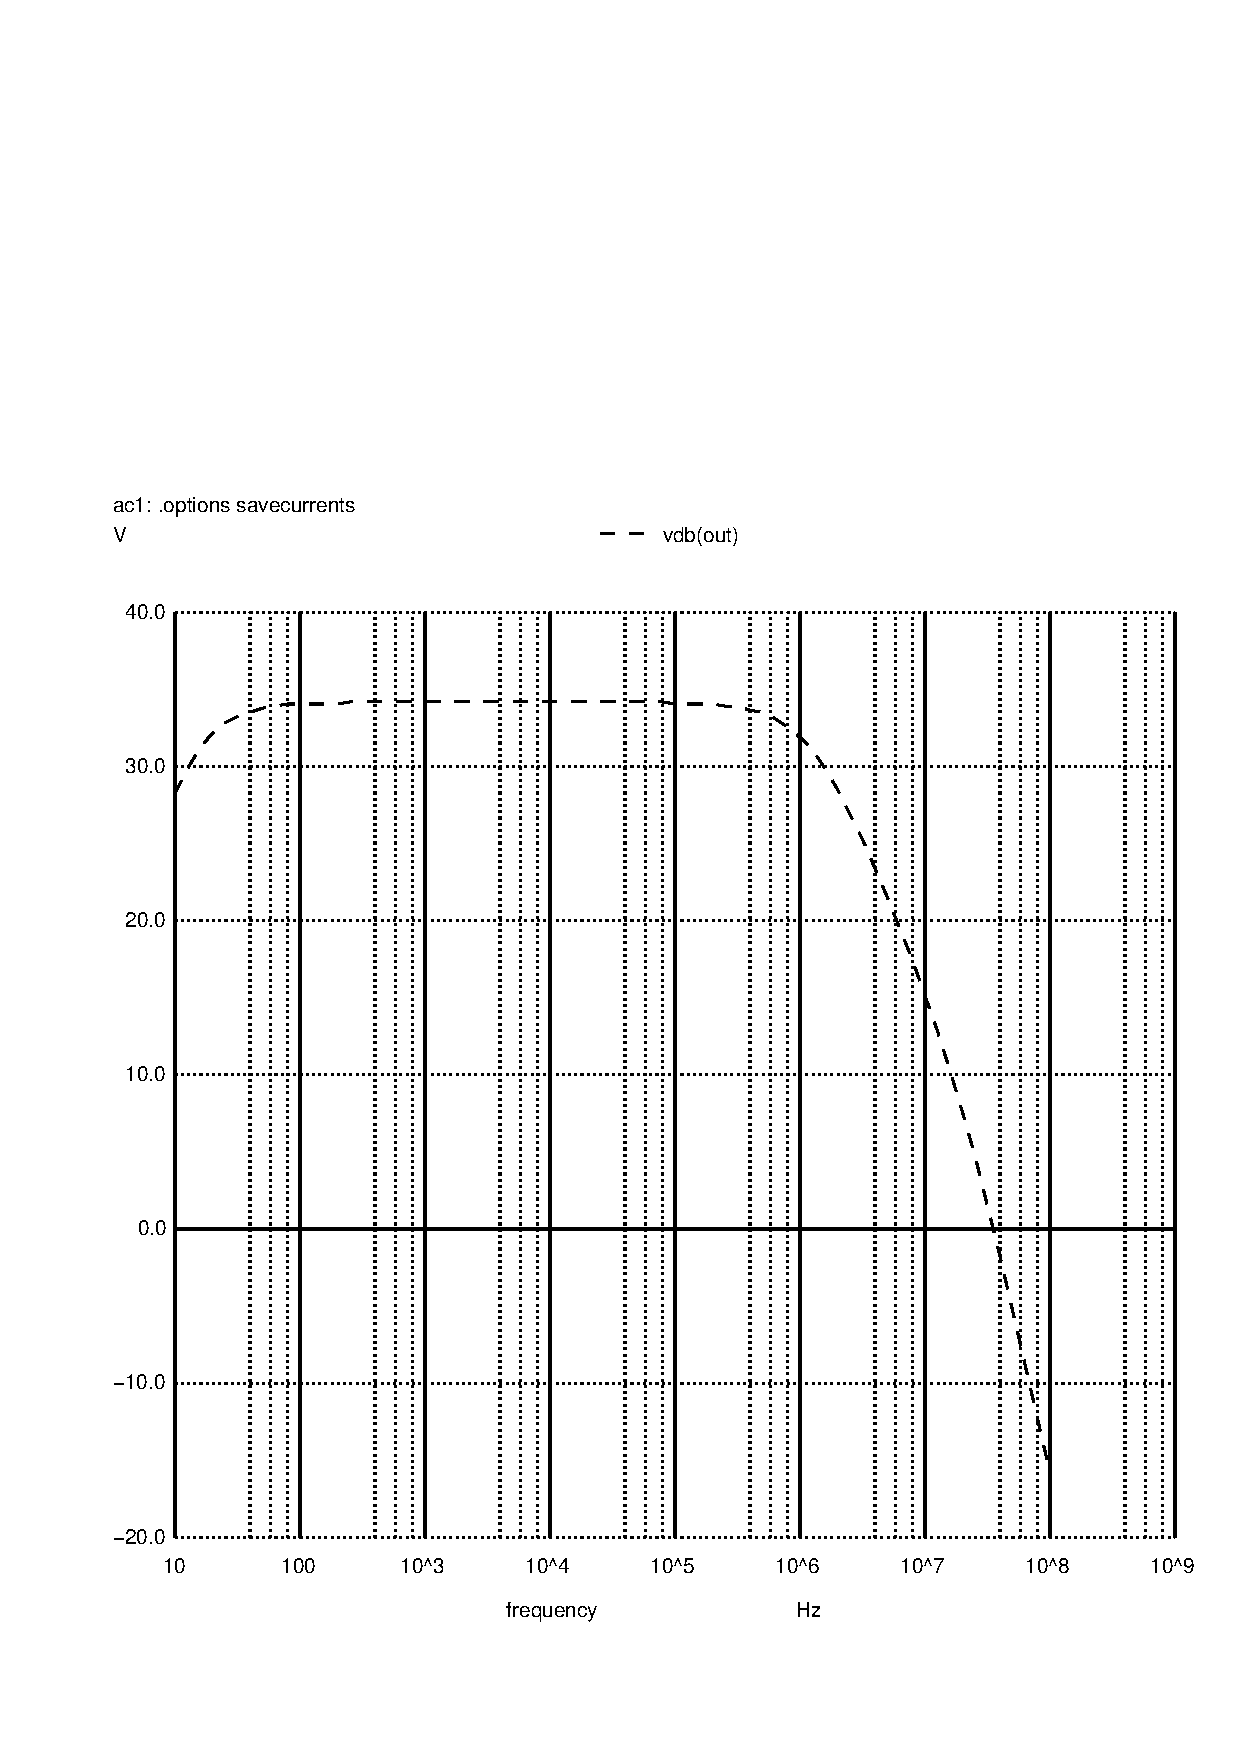
\includegraphics[width=0.7\linewidth]{vo2f.pdf}
\caption{Ngspice phase response}
\end{figure}

\begin{figure}[H] \centering
\includegraphics[width=0.7\linewidth]{teoria.eps}
\caption{Octave gain response}
\end{figure}

\begin{figure}[H] \centering
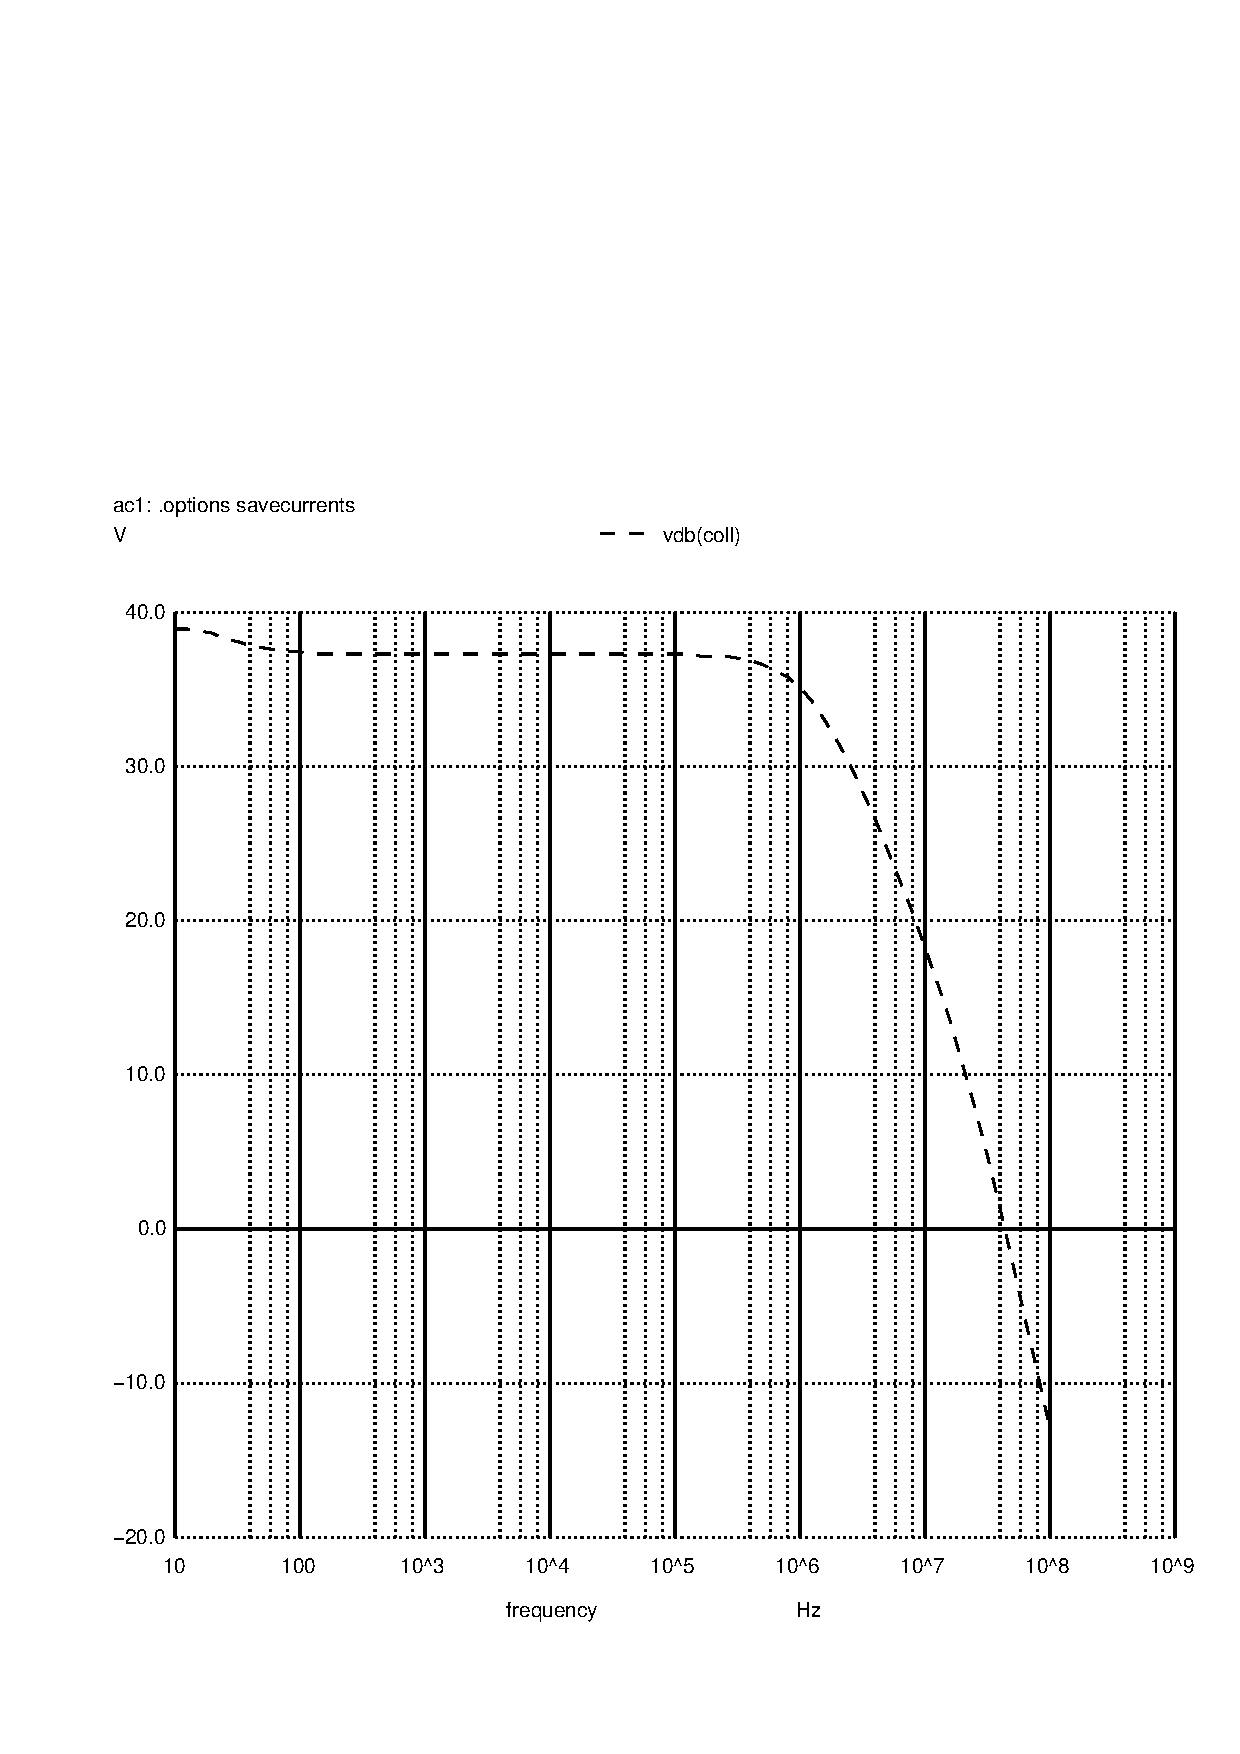
\includegraphics[width=0.7\linewidth]{vo1f.pdf}
\caption{Ngspice gain response}
\end{figure}

